%%%%%%%%%%%%%%%%%%%%%%%%%%%%% Define Article %%%%%%%%%%%%%%%%%%%%%%%%%%%%%%%%%%
\documentclass[twoside, 12pt]{report}   % two side printing
%%%%%%%%%%%%%%%%%%%%%%%%%%%%%%%%%%%%%%%%%%%%%%%%%%%%%%%%%%%%%%%%%%%%%%%%%%%%%%%

%%%%%%%%%%%%%%%%%%%%%%%%%%%%% Using Packages %%%%%%%%%%%%%%%%%%%%%%%%%%%%%%%%%%
\usepackage{geometry}
\usepackage{graphicx}
\usepackage{amssymb}
\usepackage{amsmath}
\usepackage{amsthm}
\usepackage{empheq}
\usepackage{mdframed}
\usepackage{booktabs}
\usepackage{siunitx}
\usepackage{lipsum}
\usepackage{graphicx}
\usepackage{color}
\usepackage{psfrag}
\usepackage{pgfplots}   % For plotting beautiful graphs
\usepackage{bm}
\usepackage[english]{babel}
\usepackage[backend=bibtex, sorting=none]{biblatex} %refsection=chapter
\usepackage{csquotes} 
\usepackage{setspace}
\usepackage{multicol}  
\usepackage[skip=1em plus 2pt, indent=30pt]{parskip}    % Setting space between paragraphs and indent
\usepackage[T1]{fontenc}    % Output font encoding for international characters
\usepackage{helvet}        % Selecting font family
\usepackage{ragged2e}      % For text alignment
\usepackage{caption}
\usepackage{subcaption}
\usepackage{tikz}
\usepackage[american]{circuitikz}
\usepackage{titlesec}
\usepackage{float}
\usepackage{pdfpages}
\usetikzlibrary{tikzmark,decorations.pathmorphing, shapes.geometric, shapes.symbols, arrows, shadows}
%%%%%%%%%%%%%%%%%%%%%%%%%%%%%%%%%%%%%%%%%%%%%%%%%%%%%%%%%%%%%%%%%%%%%%%%%%%%%%%

% Other Settings
%\let\cleardoublepage=\clearpage
\renewcommand{\baselinestretch}{1.5}
\setcounter{secnumdepth}{3}
\setlength\parindent{0pt}
%%%%%%%%%%%%%%%%%%%%%%%%%% Page Setting %%%%%%%%%%%%%%%%%%%%%%%%%%%%%%%%%%%%%%%
\geometry{a4paper, top=3cm, bottom=3cm, outer=3cm, inner=4cm}  % Setting page size
\graphicspath{{images/}}    % Setting path for images
\addbibresource{bibliography.bib}   % Setting path for bibliography
%%%%%%%%%%%%%%%%%%%%%%%%%% Define some useful colors %%%%%%%%%%%%%%%%%%%%%%%%%%
\definecolor{ocre}{RGB}{243,102,25}
\definecolor{mygray}{RGB}{243,243,244}
\definecolor{deepGreen}{RGB}{26,111,0}
\definecolor{shallowGreen}{RGB}{235,255,255}
\definecolor{deepBlue}{RGB}{61,124,222}
\definecolor{shallowBlue}{RGB}{235,249,255}
%%%%%%%%%%%%%%%%%%%%%%%%%%%%%%%%%%%%%%%%%%%%%%%%%%%%%%%%%%%%%%%%%%%%%%%%%%%%%%%

%%%%%%%%%%%%%%%%%%%%%%%%%% Define an orange box command %%%%%%%%%%%%%%%%%%%%%%%%
\newcommand\orangebox[1]{\fcolorbox{ocre}{mygray}{\hspace{1em}#1\hspace{1em}}}
%%%%%%%%%%%%%%%%%%%%%%%%%%%%%%%%%%%%%%%%%%%%%%%%%%%%%%%%%%%%%%%%%%%%%%%%%%%%%%%

%%%%%%%%%%%%%%%%%%%%%%%%%%%% English Environments %%%%%%%%%%%%%%%%%%%%%%%%%%%%%
\newtheoremstyle{mytheoremstyle}{3pt}{3pt}{\normalfont}{0cm}{\rmfamily\bfseries}{}{1em}{{\color{black}\thmname{#1}~\thmnumber{#2}}\thmnote{\,--\,#3}}
\newtheoremstyle{myproblemstyle}{3pt}{3pt}{\normalfont}{0cm}{\rmfamily\bfseries}{}{1em}{{\color{black}\thmname{#1}~\thmnumber{#2}}\thmnote{\,--\,#3}}
\theoremstyle{mytheoremstyle}
\newmdtheoremenv[linewidth=1pt,backgroundcolor=shallowGreen,linecolor=deepGreen,leftmargin=0pt,innerleftmargin=20pt,innerrightmargin=20pt,]{theorem}{Theorem}[section]
\theoremstyle{mytheoremstyle}
\newmdtheoremenv[linewidth=1pt,backgroundcolor=shallowBlue,linecolor=deepBlue,leftmargin=0pt,innerleftmargin=20pt,innerrightmargin=20pt,]{definition}{Definition}[section]
\theoremstyle{myproblemstyle}
\newmdtheoremenv[linecolor=black,leftmargin=0pt,innerleftmargin=10pt,innerrightmargin=10pt,]{problem}{Problem}[section]
%%%%%%%%%%%%%%%%%%%%%%%%%%%%%%%%%%%%%%%%%%%%%%%%%%%%%%%%%%%%%%%%%%%%%%%%%%%%%%%

%%%%%%%%%%%%%%%%%%%%%%%%%%%%%%% Plotting Settings %%%%%%%%%%%%%%%%%%%%%%%%%%%%%
\usepgfplotslibrary{colorbrewer}
\pgfplotsset{width=8cm,compat=1.9}
%%%%%%%%%%%%%%%%%%%%%%%%%%%%%%%%%%%%%%%%%%%%%%%%%%%%%%%%%%%%%%%%%%%%%%%%%%%%%%%

%%%%%%%%%%%%%%%%%%%%%%%%%%%%%%% Title & Author %%%%%%%%%%%%%%%%%%%%%%%%%%%%%%%%
\title{Design of a time-to-digital converter to be used as a phase detector in a PLL in 65 nm technology}
\author{Luis Guillermo Macias Rojas}
%%%%%%%%%%%%%%%%%%%%%%%%%%%%%%%%%%%%%%%%%%%%%%%%%%%%%%%%%%%%%%%%%%%%%%%%%%%%%%%

\begin{document}
    \begin{titlepage}
        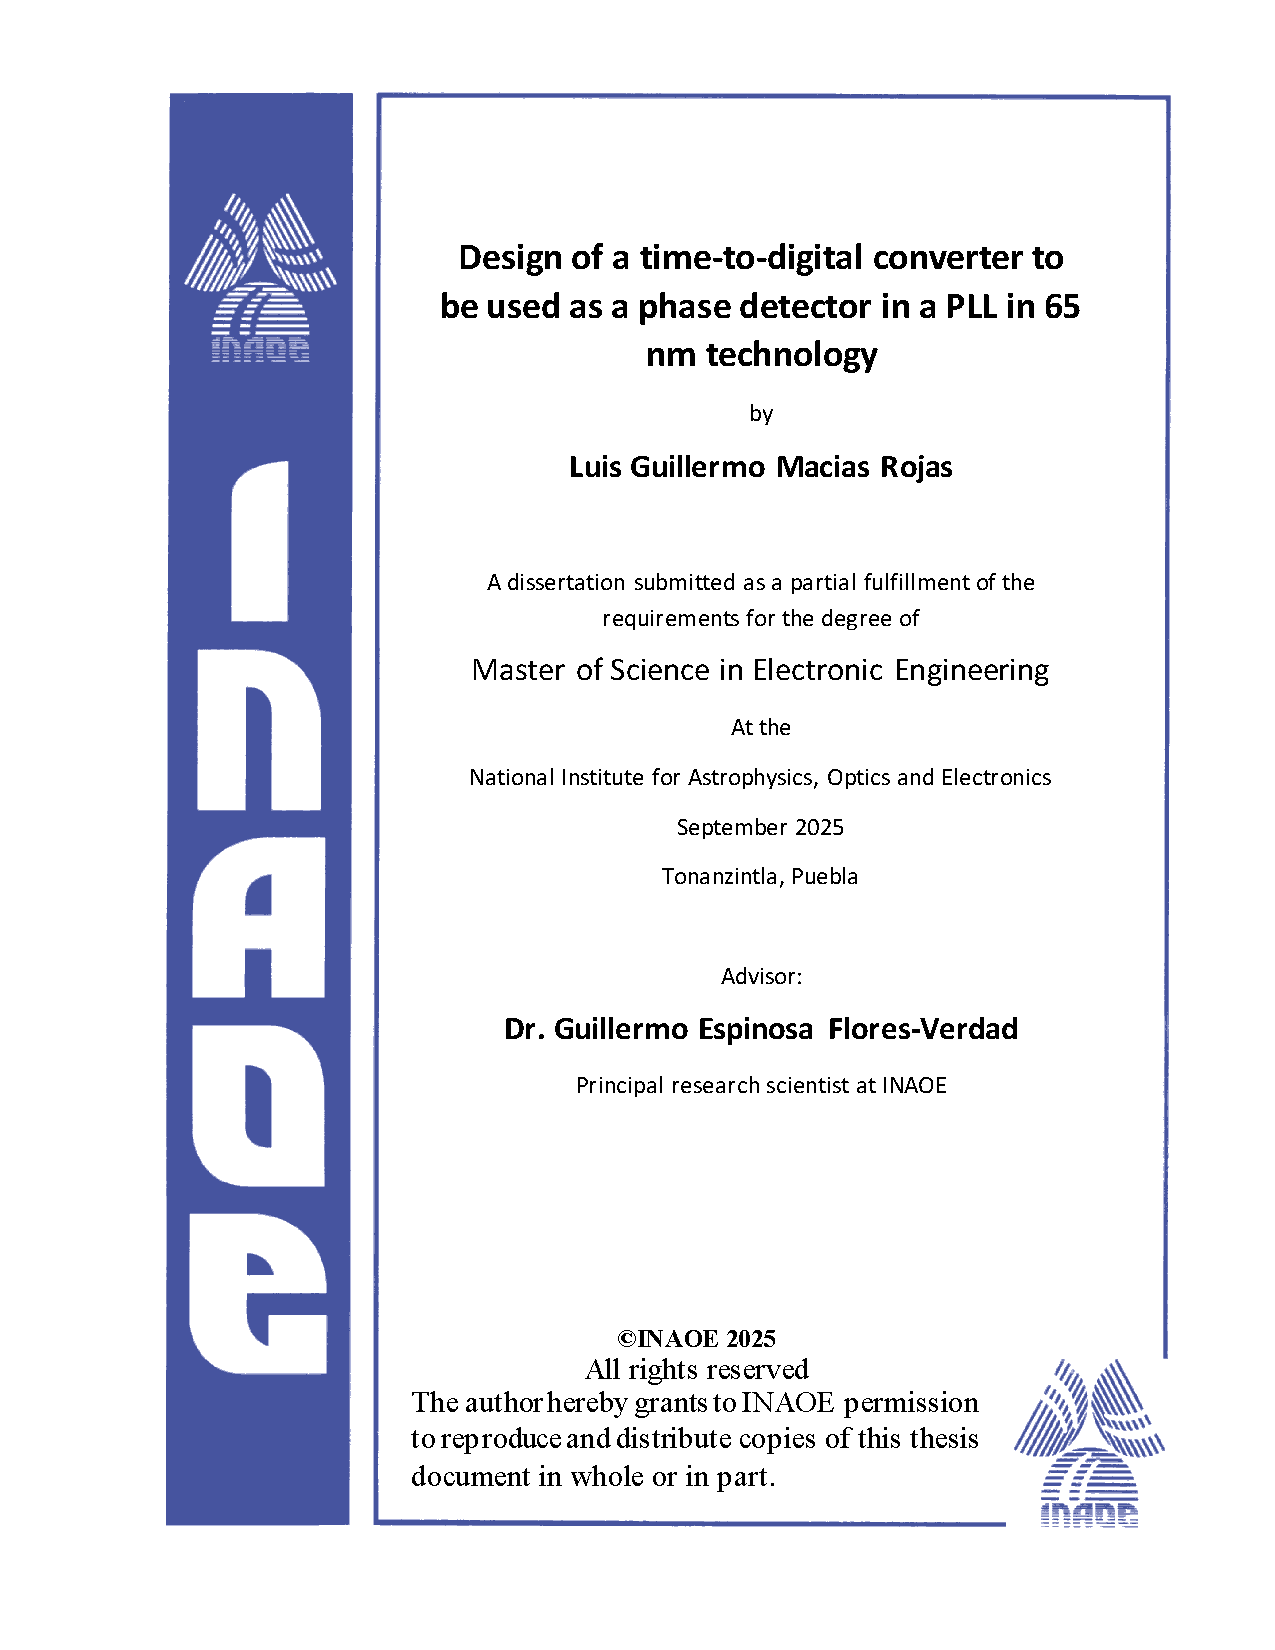
\includepdf{Portada_Tesis_Guillermo.pdf}    %Insert here PDF title page
    \end{titlepage}

    \fontfamily{phv}\selectfont % Selecting font family
    \chapter*{Resumen}
    El imparable escalamiento de la tecnología CMOS acentúa las limitaciones del diseño analógico, tales como la reducción del voltaje de alimentación, el aumento del "\textit{mismatch}"
    entre dispositivos y la degradación del rendimiento frente al ruido. Estas desventajas intrínsecas han orientado el campo de la generación estable de reloj y la síntesis de frecuencia
    hacia los "\textit{All-Digital Phase-Locked Loops}" (ADPLL). Un componente crítico de los ADPLL es el Convertidor de Tiempo a Digital (TDC), que reemplaza al tradicional detector de
    fase y frecuencia (PFD) presente en las arquitecturas analógicas. Si bien esta revolución hacia los ADPLL ha impulsado una gran innovación en el diseño de TDCs, un área que ha
    recibido una atención significativamente menor son los TDCs bipolares de línea de retardo.

    La contribución principal de esta tesis es el análisis, diseño e implementación de un novedoso TDC bipolar de 5 bits que duplica el rango dinámico intrínseco de las arquitecturas estándar.
    El TDC se complementa con un Oscilador Controlado Digitalmente (DCO) "\textit{custom}", basado en un par "\textit{cross-coupled}" y un tanque LC operando a una frecuencia central de
    7.92 GHz y que presenta un ruido de fase de -79,62 dBc/Hz a una banda lateral de 100 kHz.

    \chapter*{Abstract}
    The relentless scaling of CMOS technology exacerbates analog design limitations such as reduced supply voltage, increased device mismatch, and degraded noise performance. These
    intrinsic disadvantages have steered the field of stable clock generation and frequency synthesis toward All-Digital Phase-Locked Loops (ADPLLs). A critical component of ADPLLs is
    the Time-to-Digital Converter (TDC), which supersedes the traditional phase-frequency detector (PFD) from analog architectures. While this ADPLL revolution has spurred extensive
    innovation in TDC design, one area that has received significantly less attention is the Bipolar Delay Line TDC.

    The key contribution of this thesis is the analysis, design, and implementation of a novel 5-bit bipolar TDC that doubles the intrinsic dynamic range of standard architectures.
    The TDC is complemented by a custom Digitally-Controlled Oscillator (DCO) based on a cross-coupled pair and LC-tank operating at a center frequency of 7.92 GHz with a phase noise of
    -79.62 dBc/Hz at a 100 kHz sideband.

    \chapter*{Acknowledgements}
    First and foremost, I would like to express my deepest gratitude to my supervisor, Dr. Guillermo Espinosa Flores-Verdad, for his invaluable guidance, unwavering support,
    and immense patience throughout this research. His expertise and insightful feedback were fundamental to the completion of this work.

    I am also grateful to M.S. Erick Arenas for his advice on the DCO design.
    \chapter*{Dedications}
    To my wife and parents, for their unconditional support and love.
    %%%%%%%%%%%%%%%%% Index $$$$$$$$$$$$$$$$$$$$$$$$
    \chapter*{}
    \tableofcontents
    \listoffigures
    \addcontentsline{toc}{chapter}{List of figures}
    \listoftables
    \addcontentsline{toc}{chapter}{List of tables}

    %\input{chapters/portada.tex}
    \chapter{Introduction}
\lipsum[1-2]
    \chapter{Theoretical framework}

\section{Phase-locked loop fundamentals}
\subsection{Basic structure}
\subsection{Key PLL parameters}
\subsubsection{Phase noise / jitter}
sggs
\subsubsection{Output frequency}
It is defined as the range of frequencies that the PLL is capable of generating and can be determined by the VCO output range and the division ratio of the feedback frequency divider. This
is a key metric in establishing the application of the PLL (e.g., clock generation or RF synthesizer) and it bears significant importance in the design process due to the tradeoff 
it has with the phase noise performance of the PLL.
\subsubsection{Loop bandwidth}
\subsubsection{Noise bandwidth}
dfbdfb
\subsubsection{Lock-in time}
dnsds
\subsubsection{Pull-in time}
danan
\subsubsection{Lock-in range}
adnna
\subsubsection{Pull-in range}
anan
\subsubsection{Pull-out range}
nana
\subsubsection{Hold range}
fdan
\subsubsection{SNR}
adfn
\subsubsection{Power consumption}
dfanna
\subsubsection{Spurious tones}
fdafdhdhdah

\subsection{Analog phase-locked loops}
dfanadn
\subsection{Linearized model}
daan
\subsection{Digital phase-locked loops}
anan
\section{Time-to-digital converters}
\subsection{Delay-locked loop fundamentals}
\subsection{TDC as a phase detector}

\section{65 nm CMOS technology}

    \chapter{Literature review}
\lipsum[1-2] \cite{van1994}
    \chapter{Methodology}
\lipsum[1-2]
    \chapter{Results}
\lipsum[1-2]
    \chapter{Discussion}
\lipsum[1-2]
    \chapter{Conclusion}
\lipsum[1-2]
    %%%%%%%%%%%%%%%%%%%%%%%%%%%%%%%%%%%%%%%%%%%%%%%%
    %\appendix
    %\chapter{Appendix}
\lipsum[4]

    \printbibliography  % Print bibliography
\end{document}